\documentclass[../Funzionalita.tex]{subfiles}

\begin{document}

	\subsection{Gestione delle mappe}
	\label{subsec:GestioneMappe}
	
		\subsubsection{Panoramica}
			La funzionalità gestione mappe è resa disponibile dalle componenti del package \service, tramite questo infatti le componenti del \presenter\ e della \view\ offriranno la possibilità all'utente di effettuare operazioni sul database locale dell'applicazione. Queste operazioni sono:
			\begin{itemize}
				\item aggiunta di una mappa scaricandola da Internet;
				\item rimozione di una mappa scaricata precedentemente;
				\item aggiornamento di una mappa scaricata precedentemente.
			\end{itemize}
			Di seguito la procedura di un'aggiunta di una mappa (per la rimozione e l'aggiornamento la procedura è praticamente uguale):
			\begin{enumerate}
				\item l'utente accede alla sezione \textit{Le mie mappe} dal menu dell'applicazione;
				\item \LocalMapActivity\ richiede a \DatabaseService\ le mappe presenti nel database locale e aggiorna \LocalMapManagerViewImp\ che le mostra all'utente;
				\item  l'utente preme il pulsante in basso a destra \textit{Aggiungi mappa};
				\item \RemoteMapManagerActivity\ chiede a \DatabaseService\ le mappe disponibili online e aggiorna \RemoteMapManagerViewImp.
				\item l'utente può scegliere quale mappa scaricare, il download e il salvataggio di tale mappa scelta verrà eseguito sempre da \DatabaseService.
			\end{enumerate}
			
		\newpage
		\subsubsection{Interfaccia Grafica}
			La gestione mappe comprende due viste. La principale è \LocalMapManagerView\ che viene aperta all'accesso in tale sezione, successivamente per poter fare operazione che coinvolgono attività via Internet viene utilizzata \RemoteMapManagerView. Esse vengono gestite logicamente tramite le classi presenter \LocalMapActivity\ e \RemoteMapManagerActivity. Entrambe operano con le classi \LocalMapAdapter\ e \RemoteMapManagerAdapter\ che estendono la classe \BaseAdapter\ e gestiscono, rispettivamente, la lista delle mappe locali e remote.
			
			\paragraph*{Componenti interne}
			\begin{itemize}
			
				\item Package:
				\begin{itemize}
					\item[] \view;
				\end{itemize}
				
				\item Interfacce e classi:
				\begin{itemize}
					\item[] \LocalMapManagerView, \LocalMapManagerViewImp, \LocalMapAdapter, \RemoteMapManagerView, \RemoteMapManagerViewImp, \RemoteMapManagerAdapter;
				\end{itemize}
				
			\end{itemize}
			
			
			\paragraph*{Componenti esterne}
			\begin{itemize}
				\item Interfacce e classi SDK:
				\begin{itemize}
					\item[] \AdapterView, \BaseAdapter, \ListView, \FloatingActionButton;
				\end{itemize}
			\end{itemize}
			
			\newpage
			Nella figura \ref{fig:Navigazione-NavigationView} si indicano i seguenti widget offerti dal kit \gls{Android} SDK :
			\begin{enumerate}
				\item \Toolbar;
				\item \ListView;
				\item \FloatingActionButton;
			\end{enumerate}
		
			\begin{figure} [h]
				\centering
				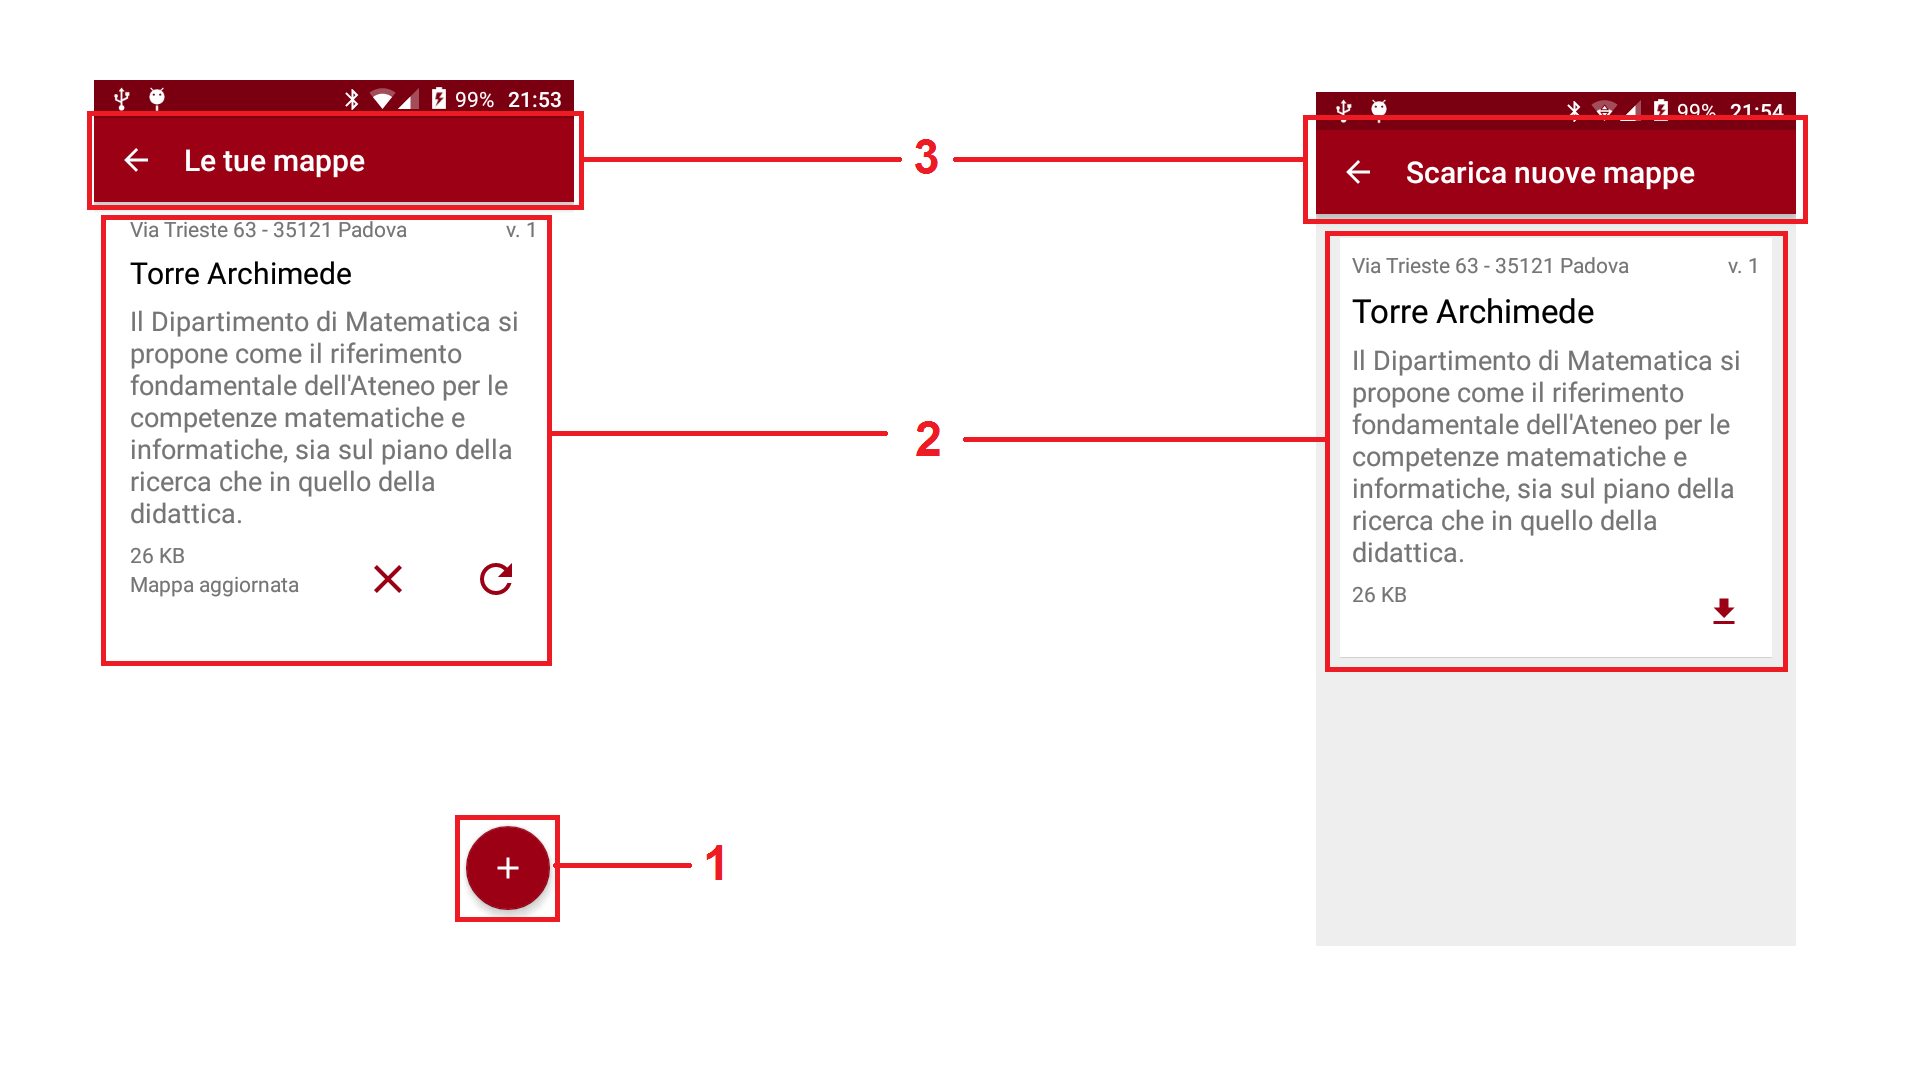
\includegraphics[scale=0.3]{img/GestioneMappe-Views}
				\caption{Gestione Mappa - Viste lista mappe locali e lista mappe remote}
				\label{fig:GestioneMappe-Views}
			\end{figure}
			
		\newpage
		\subsubsection{Presenter}
			Il compito del presenter per questa funzionalità è affidato agli oggetti \LocalMapActivity\ e \RemoteMapManagerActivity. Esse sono responsabili di gestire la logica delle view \LocalMapManagerView\ e \RemoteMapManagerView.
	
			\paragraph*{Componenti interne}
			\begin{itemize}
			
				\item Package:
				\begin{itemize}
					\item[] \view;
					\item[] \presenter;
				\end{itemize}
				
				\item Interfacce e classi:
				\begin{itemize}
					\item[] \LocalMapActivity\, \RemoteMapManagerActivity, \LocalMapManagerView\, \RemoteMapManagerView;
				\end{itemize}
				
			\end{itemize}
			
			
			\paragraph*{Componenti esterne}
			
			\begin{itemize}
				\item Interfacce e classi SDK:
				\begin{itemize}
					\item[] \Activity, \AppCompatActivity;
				\end{itemize}
			\end{itemize}
			
			
		\newpage
		\subsubsection{Download Mappe}
			Il download mappe avviene in due casi:
			\begin{itemize}
				\item l'utente ha una versione vecchia di tale mappa da scaricare (aggiornamento);
				\item l'utente non ha una versione di tale mappa da scaricare (aggiunta).
			\end{itemize}
			
			Tale operazione è eseguita dalla classe \DatabaseService\ supportata da tutte le classi con suffisso \textit{Remote} e prefisso \textit{Dao}.

			\paragraph*{Componenti interne}
			\begin{itemize}
			
				\item Package:
				\begin{itemize}
					\item[] \dataaccess;
					\item[] \service;
					\item[] \dao;
				\end{itemize}
				
				\item Interfacce e classi:
				\begin{itemize}
					\item[] \DatabaseService, \BuildingService, \EdgeService, \PhotoService, \PointOfInterestService, \RegionOfInterestService, \ServiceHelper, \CursorConverter, \SQLiteDaoFactory;\SQLDao, \BuildingDao, \CategoryDao, \EdgeDao, \EdgeTypeDao, \PhotoDao, \PointOfInterestDao, \RegionOfInterestDao, \RoiPoiDao, \RemoteBuildingDao, \RemoteCategoryDao, \RemoteEdgeDao, \RemoteEdgeTypeDao,  \RemotePhotoDao,  \RemotePointOfInterestDao, \RemoteRegionOfInterestDao, \RemoteRoiPoiDao;
				\end{itemize}
				
			\end{itemize}

\end{document}